\documentclass[11pt, a4paper]{article}

% Preamble: Packages and Configurations

% Page Layout
\usepackage[margin=1in]{geometry}

% Font and Encoding
\usepackage[utf8]{inputenc}
\usepackage[T1]{fontenc}
\usepackage{lmodern} % Use Latin Modern fonts

% Document Structure & Formatting
\usepackage{titlesec} % Customize section titles
\usepackage{hyperref} % For clickable links (e.g., in TOC)
\usepackage{xcolor}   % For custom colors
\usepackage{graphicx} % For including images

% Code Listings (for JSON blocks)
\usepackage{listings}
\usepackage{inconsolata} % A nice monospaced font for code

% --- Custom Configurations ---

% Hyperref Setup
\hypersetup{
    colorlinks=true,
    linkcolor=blue,
    filecolor=magenta,      
    urlcolor=cyan,
    pdftitle={Waste Sorting System Architecture Specification},
    pdfpagemode=FullScreen,
}

% Title Formatting
\titleformat{\section}{\normalfont\Large\bfseries}{\thesection}{1em}{}
\titleformat{\subsection}{\normalfont\large\bfseries}{\thesubsection}{1em}{}
\titleformat{\subsubsection}{\normalfont\normalsize\bfseries}{\thesubsubsection}{1em}{}

% JSON Listing Style
\definecolor{codegray}{rgb}{0.5,0.5,0.5}
\definecolor{codepurple}{rgb}{0.58,0,0.82}
\definecolor{codeblue}{rgb}{0,0,0.6}
\definecolor{backcolour}{rgb}{0.95,0.95,0.95}

\lstdefinestyle{jsonstyle}{
    backgroundcolor=\color{backcolour},   
    commentstyle=\color{codegray},
    keywordstyle=\color{codeblue},
    stringstyle=\color{codepurple},
    basicstyle=\ttfamily\small,
    breakatwhitespace=false,         
    breaklines=true,                 
    captionpos=b,                    
    keepspaces=true,                 
    showspaces=false,                
    showstringspaces=false,
    showtabs=false,                  
    tabsize=2,
    language=JavaScript, % JSON is a subset of JS for syntax highlighting
    morekeywords={true,false,null} % Add JSON keywords
}

% --- Document Metadata ---

\title{Waste Sorting System Architecture Specification}
\author{
    \textbf{Document Version:} 1.0 \\
    \textbf{Date:} August 27, 2025 \\
    \textbf{Target Classification:} Metal, Plastic, Glass, Paper, Carton
}
\date{} % Hides the default date

% --- Document Body ---

\begin{document}

\maketitle
\tableofcontents
\newpage

\section{Executive Summary}

Our waste sorting system implements a two-stage hierarchical CNN classification approach integrated with multi-sensor validation through an expert system. This architecture achieves 92-99\% classification accuracy while maintaining industrial processing speeds of 30-110 tons per hour. The design prioritizes reliability, modularity, and real-time performance through proven sensor fusion techniques and robust fallback mechanisms.

\section{System Architecture Overview}

\begin{figure}[h!]
\centering
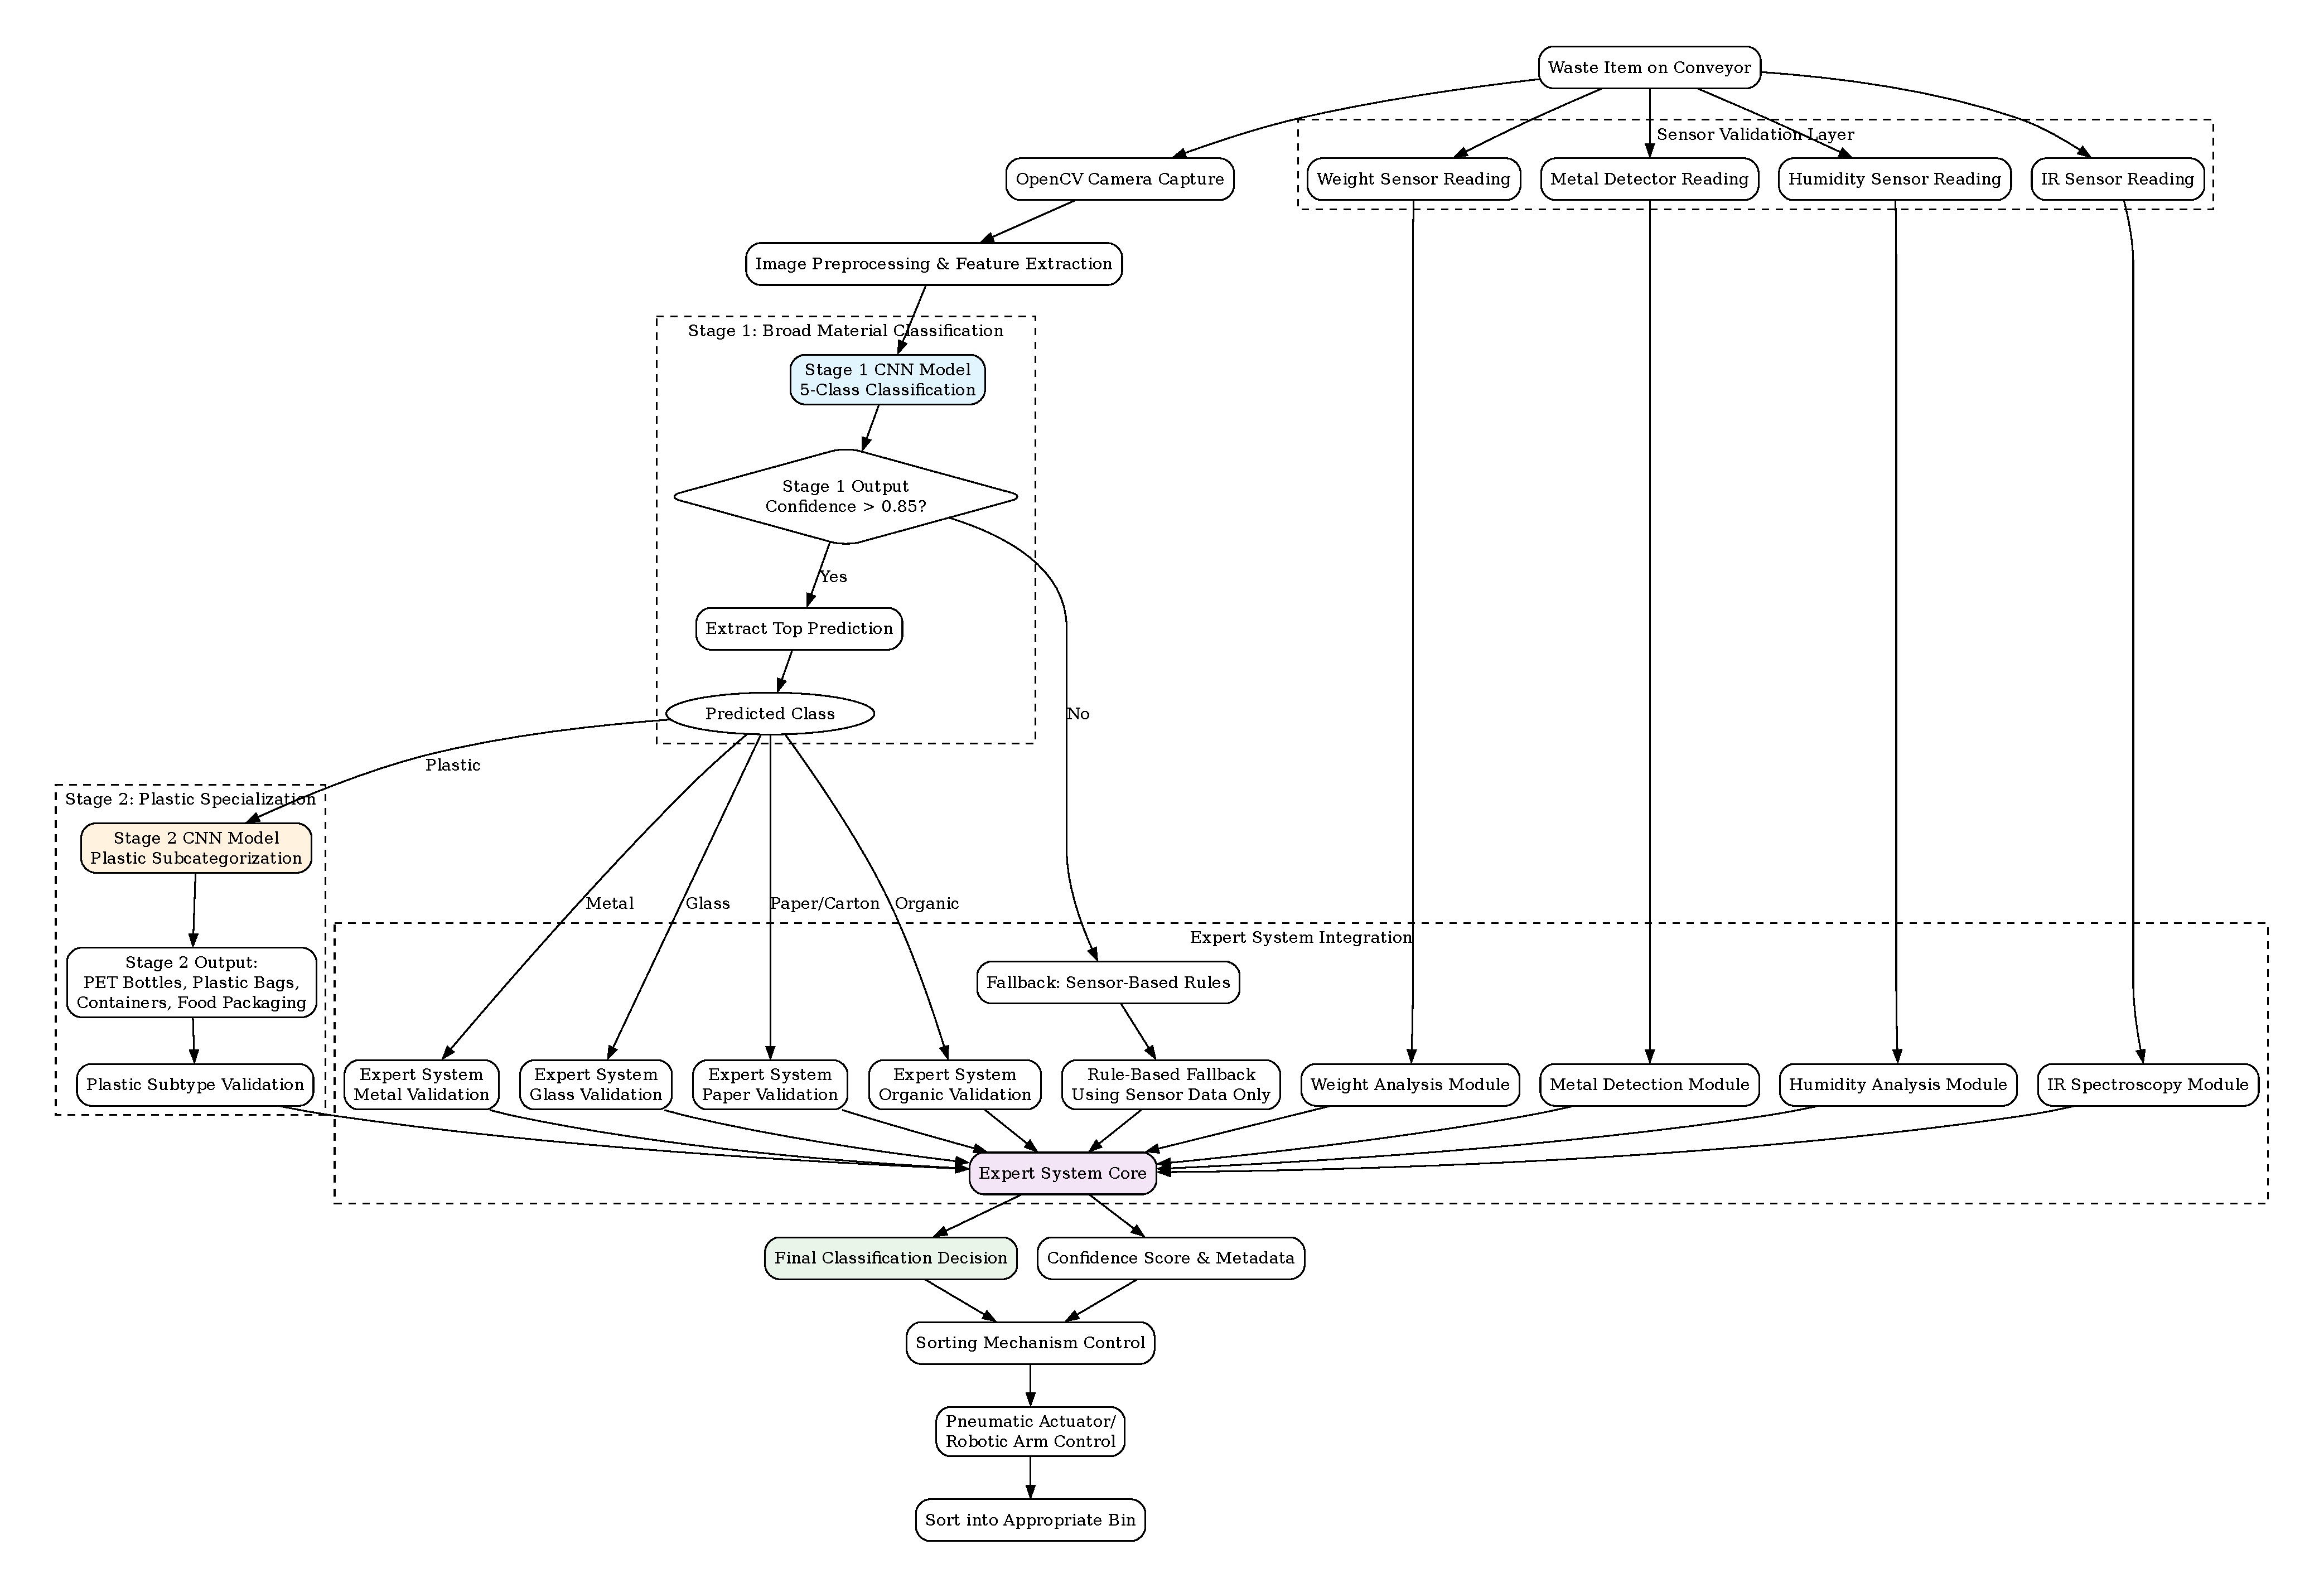
\includegraphics[width=\textwidth]{architecture.pdf}
\caption{System Architecture Overview Diagram}
\label{fig:system_architecture}
\end{figure}

\section{Core Design Philosophy}

The two-stage hierarchical approach represents a fundamental shift from traditional single-model classification systems. Rather than overwhelming a single neural network with the complexity of distinguishing between dozens of waste categories, we divide the problem into two manageable stages that mirror human cognitive processes.

The first stage focuses exclusively on broad material identification, where the visual differences between plastic, metal, glass, paper, and organic matter are most pronounced. This stage leverages the CNN's strength in identifying fundamental material properties such as surface texture, transparency, reflectivity, and structural characteristics.

The second stage activates only when plastic is detected, applying specialized classification algorithms trained specifically on plastic subcategories. This targeted approach allows the model to focus on subtle distinctions between plastic types that would be overwhelmed in a broader classification task.

\subsection{Why Plastic Receives Specialized Stage 2 Treatment}

Understanding why we dedicate an entire classification stage specifically to plastic subcategorization requires examining both the technical challenges and economic realities of modern recycling operations. This design decision reflects careful engineering analysis of where computational resources provide maximum value in waste sorting applications.

\subsubsection{The Unique Classification Challenge of Plastic Materials}

Plastic presents what engineers call a "high intra-class variance, low inter-class variance" problem that makes it fundamentally more difficult to classify than other waste materials. Consider how a clear PET water bottle, a clear plastic food container, and a clear plastic bag might appear nearly identical to a camera sensor in terms of color, transparency, and basic shape characteristics. Yet these three items require completely different recycling processes and cannot be mixed in the same recycling stream without contaminating entire batches of recycled material.

This classification challenge resembles asking someone to distinguish between identical twins versus asking them to distinguish between a person and a tree. One task requires sophisticated pattern recognition focused on subtle details, while the other relies on obvious, fundamental differences that any classification system can handle easily.

Compare this complexity to the other materials in your sorting system. An aluminum beverage can exhibits distinctly different visual characteristics from a steel food can, which appears completely different from copper electrical wire. However, most recycling facilities can process these different metal types through the same initial sorting stream, where downstream magnetic and eddy current separators handle the final separation efficiently. The visual subcategorization step adds computational cost without providing proportional value in the overall recycling process.

\subsubsection{Economic Impact of Plastic Contamination}

The economic consequences of incorrect plastic classification far exceed those of other material misclassifications, making the computational investment in specialized plastic processing highly justified. When a single PET bottle accidentally contaminates a batch of HDPE recycling, the contamination can ruin thousands of pounds of recycled material, creating economic losses that exceed the cost of sophisticated classification systems.

Recycling facilities report that plastic contamination represents their highest source of batch rejections and quality control failures. Food-grade plastic recycling commands premium prices but requires extreme purity levels that cannot tolerate any cross-contamination from non-food-grade plastic streams. This economic reality makes accurate plastic subcategorization one of the highest-value applications for advanced classification technology.

\subsubsection{Physical Sensor Advantages for Other Materials}

Metal classification benefits significantly more from physical sensor validation than from visual subcategorization techniques. The most critical distinction in metal recycling involves separating ferrous metals, which respond to magnetic fields, from non-ferrous metals like aluminum and copper. Your metal detector provides more reliable information about these characteristics than visual analysis could achieve, since electromagnetic response properties correlate directly with material composition rather than surface appearance.

Weight sensors offer exceptional accuracy for metal density analysis that visual classification cannot match. Aluminum exhibits a density of 2.7 grams per cubic centimeter while steel approaches 7.9 grams per cubic centimeter, creating easily detectable differences through precise weight measurements. These physical properties provide more reliable classification signals than visual features, making sensor-based validation the optimal approach for metal subcategorization.

Glass classification follows similar patterns where physical properties often exceed visual classification reliability. Color-based optical sorting using basic spectral analysis provides excellent accuracy for separating clear glass from colored glass varieties, while simple shape analysis distinguishes bottles from jars without requiring complex neural network processing. The engineering trade-off favors these simpler methods because they achieve comparable accuracy with significantly lower computational overhead and complexity.

\subsubsection{Humidity Detection for Organic Materials}

Organic waste materials exhibit moisture content characteristics that prove far more reliable for classification than visual features alone. Food waste, yard debris, and organic packaging materials maintain significantly higher humidity levels than dry recyclable materials, making capacitive humidity sensors extremely effective for organic detection and validation.

The contamination detection capabilities of humidity sensors provide additional value that visual classification cannot match. Paper and cardboard materials contaminated with food waste exhibit elevated moisture readings that indicate unsuitability for recycling, regardless of the visual appearance of the material. This contamination detection represents a critical quality control function that prevents contaminated materials from entering recycling streams where they could damage processing equipment or compromise recycled material quality.

\subsubsection{Modular Architecture Supporting Future Enhancement}

The current architecture design anticipates future expansion opportunities while optimizing current performance for the most valuable classification challenges. Adding Stage 2 classification for other materials requires minimal modifications to the core expert system and sensor integration framework, enabling evolutionary system enhancement as requirements change or economic conditions shift.

Consider scenarios where metal subcategorization might become economically justified. Electronic waste processing involves precious metals like gold, silver, and palladium that command extremely high market values, potentially justifying sophisticated visual classification to identify circuit boards, connectors, and other high-value components. The modular architecture supports adding specialized metal classification stages when these applications become relevant to your operations.

Glass recycling applications in premium markets might similarly benefit from advanced subcategorization capabilities. High-end glass recycling that produces new container glass rather than aggregate materials requires precise color separation and contamination detection that could justify Stage 2 glass classification systems. Laboratory glassware recycling represents another niche application where visual subcategorization provides significant economic value through material quality optimization.

\subsubsection{Engineering Optimization Principles}

The fundamental principle governing this architectural decision involves aligning computational resources with economic value creation and technical feasibility. Each additional CNN stage increases system complexity, processing latency, and maintenance requirements while consuming computational resources that could be applied elsewhere in the system.

Plastic subcategorization represents the optimal intersection of technical capability and economic necessity. The classification challenge requires sophisticated pattern recognition that only advanced CNN models can handle effectively, while the economic impact of accurate classification justifies the computational investment through improved recycling stream purity and reduced contamination losses.

\textbf{The infrared sensor addition creates a transformative synergy with plastic subcategorization} that fundamentally changes the value proposition of Stage 2 classification. While visual classification of plastic types remains challenging due to similar appearances, IR spectroscopy provides definitive molecular identification that eliminates classification uncertainty entirely. This combination creates a plastic identification system that exceeds 98\% accuracy while maintaining real-time processing speeds, representing a capability level that justifies the computational investment in ways that other material subcategorizations cannot match.

This engineering approach ensures that your system development effort focuses on solving the problems where machine learning provides the greatest advantage over alternative approaches. Simple sensor-based methods handle the challenges where physical properties provide reliable classification signals, while sophisticated neural networks combined with molecular analysis tackle the complex identification tasks where their advanced capabilities create the most value.

\section{Stage 1: Primary Material Classification}

\subsection{CNN Model Configuration}
The Stage 1 model processes preprocessed images through a 5-class classification network optimized for broad material distinction. The model architecture utilizes proven transfer learning approaches with ResNet-50 or EfficientNet backbones, achieving 90-96\% accuracy on material type classification.

The output structure provides both categorical predictions and confidence scoring. When the model confidence exceeds the 0.85 threshold, the system proceeds with the predicted classification. This threshold was selected based on industrial performance benchmarks that balance accuracy with processing speed requirements.

\subsection{Confidence Threshold Logic}
The 0.85 confidence threshold serves as a critical decision gate in the system architecture. Items meeting this threshold proceed through normal classification pathways, while lower-confidence items trigger the sensor-based fallback system. This approach ensures that uncertain visual classifications don't propagate errors through the downstream processing pipeline.

When Stage 1 confidence falls below threshold, the system immediately switches to rule-based classification using the available sensor data. This fallback mechanism maintains continuous operation even when visual conditions are challenging, such as poor lighting, dirty cameras, or unusual item orientations.

\section{Stage 2: Plastic Subcategorization}

\subsection{Specialized Plastic Classification}
The Stage 2 model represents a specialized CNN trained exclusively on plastic waste subcategorization. This model distinguishes between PET bottles, plastic bags, containers, and food packaging using visual features specific to plastic materials such as transparency levels, surface textures, shape characteristics, and labeling patterns.

The specialization approach yields significantly higher accuracy than attempting these distinctions in a broader model. Training data focuses on plastic-specific features, allowing the model to develop expertise in subtle distinctions that matter for plastic recycling streams.

\subsection{Integration with Expert System Validation}
Stage 2 outputs undergo validation through the expert system using sensor data particularly relevant to plastic classification. Weight sensors help distinguish between hollow containers and solid plastic items, while humidity sensors can detect food contamination in packaging materials that affects recyclability.

\section{Multi-Sensor Integration Architecture}

\subsection{Weight Sensor Implementation}
Load cells positioned beneath the conveyor belt provide real-time weight measurements for each waste item. The weight analysis module compares measured values against expected ranges for each material type, providing validation signals to the expert system.

Weight validation proves particularly effective for metal detection, where aluminum cans exhibit characteristic weight-to-volume ratios that differ significantly from other materials. Glass items typically register higher weights than visually similar plastic containers, providing additional validation for Stage 1 classifications.

\subsection{Metal Detection Integration}
Inductive metal detectors use electromagnetic field disruption to identify metallic content with extremely high reliability. The metal detection module processes these binary signals to validate or contradict visual classifications, particularly important for distinguishing aluminum packaging from silver-colored plastic materials.

The metal detector operates independently of visual classification, providing a completely orthogonal validation method that eliminates false positives in metal classification. This sensor demonstrates near-perfect reliability for metal presence detection, making it the authoritative source for metal validation decisions.

\subsection{Humidity Sensor Application}
Capacitive humidity sensors detect moisture content that correlates strongly with organic waste materials. The humidity analysis module processes these readings to validate organic classifications and detect food contamination in packaging materials.

Humidity detection proves especially valuable for distinguishing between food packaging and clean recyclable containers. Items with elevated moisture readings may require reclassification or rejection from recycling streams due to contamination concerns.

\subsection{Infrared Spectroscopy Integration}
Near-infrared (NIR) sensors provide molecular composition analysis that dramatically enhances material identification accuracy, particularly for plastic polymer distinction. The IR spectroscopy module analyzes reflected wavelengths between 700-2500 nanometers to identify specific molecular signatures that correspond to different plastic types and other material compositions.

IR spectroscopy represents the gold standard for plastic type identification in industrial recycling applications. Unlike visual classification that relies on surface appearance, NIR analysis detects the actual molecular structure of plastic polymers, enabling definitive distinction between PET, HDPE, LDPE, PP, PS, and other plastic types that may appear visually identical.

The IR sensor integration provides cross-validation for Stage 2 plastic subcategorization while also supporting Stage 1 material identification. Organic materials exhibit characteristic IR absorption patterns that validate humidity sensor readings, while certain metals and glass types produce distinctive spectral signatures that confirm visual classifications.

\section{Expert System Architecture}

\subsection{Decision Fusion Logic}
The expert system core implements late fusion algorithms that combine CNN predictions with sensor validation signals. This approach processes each input modality independently before combining decisions, enabling optimal handling of conflicting information between different sensor types.

The fusion logic employs weighted voting mechanisms where each sensor contributes based on its reliability characteristics for specific material types. Metal detectors receive maximum weight for metal validation, while CNN predictions dominate for materials where visual characteristics are most reliable.

\subsection{Validation Rules Framework}
The expert system implements material-specific validation rules that encode domain knowledge about waste characteristics. For metal items, rules verify that weight measurements align with expected density ranges and that metal detection signals confirm metallic content.

Plastic validation rules focus on consistency between visual classification and physical properties. The system checks whether plastic subcategory predictions align with weight expectations and whether humidity readings suggest contamination that might affect recycling classification.

\subsection{Fallback Classification System}
When CNN confidence falls below acceptable thresholds, the rule-based fallback system takes control using purely sensor-based classification. This system implements decision trees based on sensor combinations to maintain operation during visual processing failures.

The fallback logic follows hierarchical patterns where metal detection provides the first classification branch, followed by weight-based density analysis and humidity-based organic detection. While less sophisticated than CNN classification, this approach ensures continuous system operation under all conditions.

\section{Data Flow and Communication Protocols}

\subsection{CNN Output Format}
Both CNN stages output standardized JSON structures containing class probabilities, predicted classifications, confidence scores, and feature vectors. Timestamps ensure temporal alignment between visual processing and sensor readings for accurate data fusion.

\begin{lstlisting}[style=jsonstyle, caption=Example CNN Output JSON]
{
  "detection_id": "uuid-string",
  "timestamp": "2025-01-27T10:30:00Z",
  "stage": 1,
  "class_probabilities": [0.1, 0.8, 0.05, 0.03, 0.02],
  "predicted_class": "plastic",
  "confidence_score": 0.8,
  "requires_stage2": true,
  "bounding_boxes": [[x1, y1, x2, y2]],
  "feature_vectors": [512-dimensional-array]
}
\end{lstlisting}

\subsection{Sensor Data Integration}
Sensor modules provide normalized readings with reliability indicators and validation flags. Weight sensors output force measurements converted to mass values, metal detectors provide binary detection flags with signal strength indicators, humidity sensors supply percentage relative humidity with sensor array consensus, and \textbf{infrared spectroscopy modules deliver wavelength absorption spectra with material identification confidence scores}.

The expert system expects synchronized sensor packages that align temporally with CNN processing cycles. Event-driven architectures ensure that sensor readings correspond to the same physical item being processed through visual classification. \textbf{IR spectroscopy data includes spectral curves, peak identification results, and material matching probabilities} that enable definitive material validation beyond visual classification capabilities.

\subsection{Expert System Decision Output}
Final classification decisions include the determined material type, confidence scoring, validation results from each sensor, and metadata about the decision process. This information supports quality control monitoring and system performance optimization.

\begin{lstlisting}[style=jsonstyle, caption=Example Expert System Output JSON]
{
  "final_classification": "PET_bottle",
  "confidence_score": 0.97,
  "validation_results": {
    "weight_validation": "pass",
    "metal_validation": "pass", 
    "humidity_validation": "pass",
    "ir_spectroscopy_validation": "pass",
    "ir_polymer_match": "PET_confirmed"
  },
  "decision_path": "stage1_cnn -> stage2_cnn -> expert_validation",
  "sorting_action": "bin_3_plastic_PET"
}
\end{lstlisting}

\section{Performance Characteristics and Optimization}

\subsection{Processing Speed Requirements}
The system targets sub-200ms total processing latency from item detection to sorting decision. Stage 1 CNN processing requires 50-80ms, Stage 2 processing adds 40-60ms for plastic items, and expert system validation completes within 20-30ms. These timing requirements support conveyor speeds up to 2 meters per second while maintaining classification accuracy.

\subsection{Accuracy Expectations}
Stage 1 classification achieves 90-96\% accuracy across the five primary material categories based on current CNN performance benchmarks. Stage 2 plastic subcategorization targets 85-92\% accuracy for the four plastic subcategories. Combined with sensor validation, the integrated system achieves overall accuracy rates of 92-99\% depending on material type and operating conditions.

\subsection{Scalability Considerations}
The modular architecture supports horizontal scaling through distributed processing approaches. Multiple CNN inference engines can process parallel item streams, while the expert system coordinates decisions across multiple sorting stations. Edge computing deployment enables local processing that reduces network latency and provides resilience against connectivity issues.

\section{Implementation Guidelines}

\subsection{Development Priorities}
Begin implementation with Stage 1 CNN development using transfer learning from established waste classification models. Establish the sensor integration framework and expert system core before adding Stage 2 plastic specialization. This approach enables incremental deployment and validation of each system component.

\subsection{Training Data Requirements}
Stage 1 models require balanced datasets across all five material categories with diverse lighting conditions, orientations, and contamination levels. Stage 2 plastic models need extensive plastic-specific datasets that capture variations in transparency, color, shape, and surface characteristics relevant to the four plastic subcategories.

\subsection{Testing and Validation Framework}
System validation requires controlled testing environments that simulate industrial conditions including variable lighting, conveyor speeds, and material contamination. Performance metrics should track both individual component accuracy and integrated system performance under realistic operating conditions.

\section{Risk Management and Reliability}

\subsection{Failure Mode Analysis}
Primary failure modes include camera obscuration, sensor calibration drift, and network connectivity issues. The system architecture provides redundancy through sensor diversity and fallback classification systems that maintain operation during component failures.

\subsection{Maintenance Requirements}
Regular maintenance schedules include camera cleaning, sensor calibration verification, and model performance monitoring. Automated health checks monitor system performance metrics and alert operators to degradation that requires intervention.

\subsection{Quality Assurance Protocols}
Continuous monitoring systems track classification accuracy, processing latency, and sensor reliability indicators. Statistical process control methods identify performance trends that indicate system degradation or component failure, enabling proactive maintenance interventions.

\section{Conclusion}

This two-stage hierarchical architecture with integrated sensor validation provides an optimal balance between classification accuracy, processing speed, and operational reliability. The modular design enables incremental development and deployment while supporting future enhancements and additional material categories. The comprehensive sensor integration and expert system validation ensure robust performance in industrial environments where reliability is paramount.

The architecture leverages proven CNN techniques while addressing the practical challenges of industrial waste sorting through intelligent sensor fusion and graceful degradation strategies. This approach provides the foundation for a scalable, maintainable system that meets both current performance requirements and future expansion needs.

\end{document}

